%%%%%%%%%%%%%%%%%%%%%%%%%%%%%%%%%%%%%%%%%%%%%%%%%%%%%%%%%%%%%%%%%%%%%%%%%%%%%%%%
%2345678901234567890123456789012345678901234567890123456789012345678901234567890
%        1         2         3         4         5         6         7         8

\documentclass[letterpaper, 10 pt, conference]{ieeeconf}  % Comment this line out
                                                          % if you need a4paper
%\documentclass[a4paper, 10pt, conference]{ieeeconf}      % Use this line for a4
                                                          % paper

\IEEEoverridecommandlockouts                              % This command is only
                                                          % needed if you want to
                                                          % use the \thanks command
\overrideIEEEmargins
\usepackage{url}
\usepackage{graphicx}

% See the \addtolength command later in the file to balance the column lengths
% on the last page of the document



% The following packages can be found on http:\\www.ctan.org
%\usepackage{graphics} % for pdf, bitmapped graphics files
%\usepackage{epsfig} % for postscript graphics files
%\usepackage{mathptmx} % assumes new font selection scheme installed
%\usepackage{times} % assumes new font selection scheme installed
%\usepackage{amsmath} % assumes amsmath package installed
%\usepackage{amssymb}  % assumes amsmath package installed

\title{\LARGE \bf
Need for Speed: Effects of Containerization on Network Performance
}

%\author{ \parbox{3 in}{\centering Huibert Kwakernaak*
%         \thanks{*Use the $\backslash$thanks command to put information here}\\
%         Faculty of Electrical Engineering, Mathematics and Computer Science\\
%         University of Twente\\
%         7500 AE Enschede, The Netherlands\\
%         {\tt\small h.kwakernaak@autsubmit.com}}
%         \hspace*{ 0.5 in}
%         \parbox{3 in}{ \centering Pradeep Misra**
%         \thanks{**The footnote marks may be inserted manually}\\
%        Department of Electrical Engineering \\
%         Wright State University\\
%         Dayton, OH 45435, USA\\
%         {\tt\small pmisra@cs.wright.edu}}
%}

\author{Swathi Hoysala, Jeyavaishnavi Muralikumar, Ashrith Sheshan % <-this % stops a space
}


\begin{document}



\maketitle
\thispagestyle{empty}
\pagestyle{empty}


%%%%%%%%%%%%%%%%%%%%%%%%%%%%%%%%%%%%%%%%%%%%%%%%%%%%%%%%%%%%%%%%%%%%%%%%%%%%%%%%


%%%%%%%%%%%%%%%%%%%%%%%%%%%%%%%%%%%%%%%%%%%%%%%%%%%%%%%%%%%%%%%%%%%%%%%%%%%%%%%%
\section{INTRODUCTION}
In recent times, software iterations are moving at a very fast pace. Computing environments running these softwares or libraries have to update to the newer iterations. Due to these updates, running softwares reliably when moved from computing environment to another becomes a huge problem.
\\
There was a need for technology that is platform/compute environment agnostic. This is where Container technology comes into picture. Container technology has gained tremendous popularity since it enables a fast and easy way to package, distribute and deploy applications and services.\\
A container consists of an entire runtime environment: an application, plus all its dependencies, libraries and other binaries, configuration files needed to run it, all bundled into one package. By containerizing the application platform and its dependencies, differences in OS distributions and underlying infrastructure are abstracted away. \\
However, networking between containers may come with its own overheads. Even between containers on the same host, different practices have different implications for performance (see related work) and we could find only a limited amount of evaluation of network performances in containerized and virtualized environments. Therefore, we plan to extend what we could find in order to better understand the effects of containerization on network performance. 

\section{RELATED WORK}

It is generally accepted that containerization imposes overheads on network performance when compared to native OS-level networking. \cite{morabito2015hypervisors} makes a comparison of hypervisors and containers in terms of several system functions, including networking performance, and conclude that Docker and LXC provide comparable throughput to native networking for TCP streams, but only 60\% of the bandwidth for UDP stream. They also measure performance and conclude that container networking degrades performance by a significant percentage.

\cite{zhao2017performance} gives a lower level and more detailed analysis of container network performance, including throughput and performance evaluation on a variety of combinations of containers, VMs and hosts, such as containers on the same host, containers on different hosts with one on a VM and so on. They make several conclusions, such as that containers on Linux are better than those on Windows, networking overhead depends on choice of network virtualization such as veth vs MACVLAN, and that VMs may or may not be better for performance since they introduce NUMA binding but also  introduce overheads. \cite{yu2016freeflow} also discusses some causes of performance limitations in container environments, such as the fact that the throughput of overlay networking between containers on a host will be limited by CPU.
\section{Initial Experiments}
We ran initial set of experiments to measure TCP and UDP latencies and bandwidths. We compared the network performance of TCP and UDP by benchmarking container-to-VM communication against VM-to-VM communication. We used tools like qperf \cite{qperf} and netperf \cite{netperf} for our measurements.
\\ The following environment was used to run the experiments:
\begin{itemize}
\item AWS - For two VMs
\item VMs running Ubuntu Server 16.04
\item RAM - 2GB
\item Storage - 20GB
\item Dokcer Version - 17.12.0-ce
\item Docker image - ubuntu:latest(17.10)
\end{itemize}
The following initial observations were made:
\begin{itemize}
\item TCP latency of container-to-VM was comparable with that of the VM-to-VM
\item TCP bandwidth of the container-to-VM was half of that of the VM-to-VM
\item Reported UDP bandwidth is much higher with containerization because it somehow leads to 100 \% CPU utilization. This does not happen for TCP.
\item UDP latency seems to suffer by a factor of 2-3.
\end{itemize}
\begin{figure}[h]
 \centering
 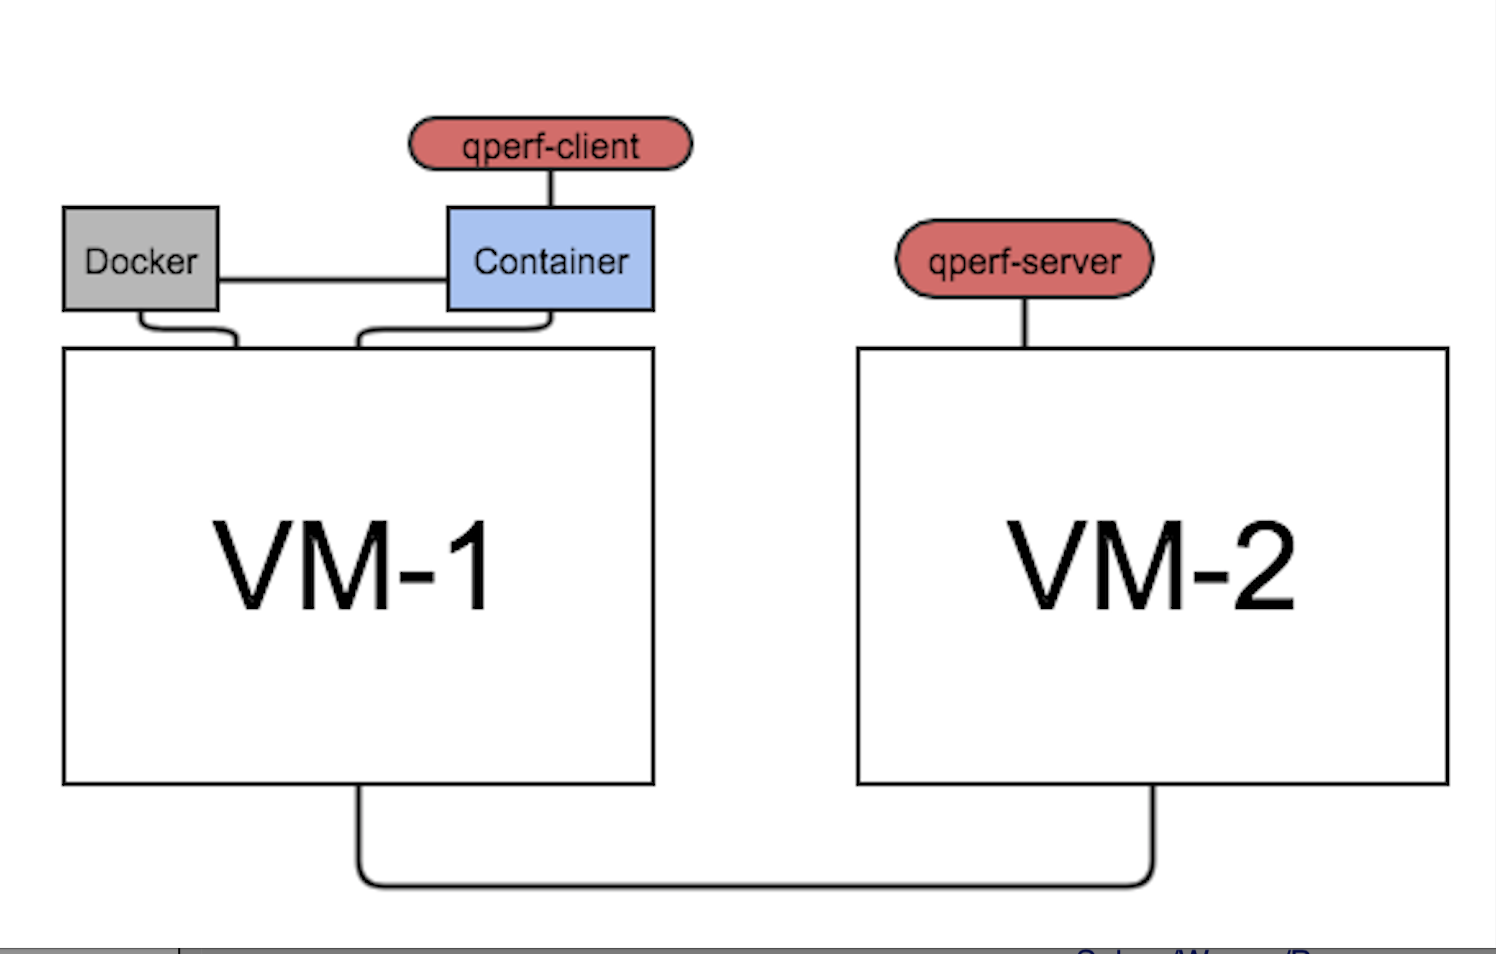
\includegraphics[width=0.5\textwidth]{cont-vm.png}
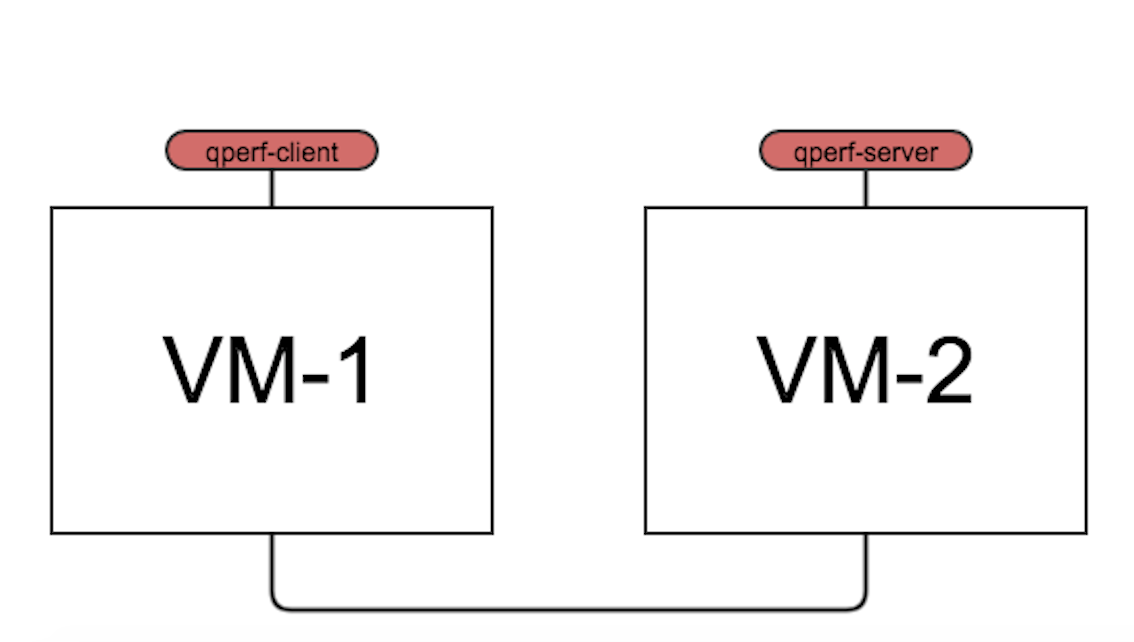
\includegraphics[width=0.5\textwidth]{vm-vm.png}
\caption{Testbed architecture used in initial experiments}
\end{figure}


\section{PLAN}
%For our evaluation we intend to create different scenarios of network overheads in a containerized application and benchmark the network performance on metrics like and bandwidth

We plan to focus our evaluations on the following questions:
\begin{enumerate}
	\item Do conclusions based on the evaluation of LXC \cite{zhao2017performance} necessarily generalize to different container images?
    \item What overhead does containerization introduce on top of virtualization?
    \item Does the network performance of containers depend on the underlying OS of the host?
\end{enumerate}
Based on the observations from our initial experiments we plan to evaluate 
\begin{enumerate}
	\item How can the disparity in UDP and TCP performance overhead be explained?
    \item What causes the container to use 100\% CPU when benchmarking UDP performance which doesn't seem to happen with TCP?
    \item How does the TCP and UDP implementation on docker scale with the number of containers running on a single host?
\end{enumerate}

\section{RESOURCES}
We currently have a couple of hundred dollars of Amazon Web Services(AWS) credits. We did our initial benchmarking on them and we see a lot of inconsistencies with the numbers we are getting. We believe that this is because of the underlying network provided by AWS.\\
In order to run our experiments correctly, we need 2 servers with the following requirements:
\begin{itemize}
\item RAM : At least 4GB
\item Storage : At least 20GB
\item Network : Ethernet
\end{itemize}
In order to compare network performance with and without containers on different operating systems(OS), we need 2 servers/hardware with OS installation capabilities. 
\addtolength{\textheight}{-12cm}   % This command serves to balance the column lengths
                                  % on the last page of the document manually. It shortens
                                  % the textheight of the last page by a suitable amount.
                                  % This command does not take effect until the next page
                                  % so it should come on the page before the last. Make
                                  % sure that you do not shorten the textheight too much.

%%%%%%%%%%%%%%%%%%%%%%%%%%%%%%%%%%%%%%%%%%%%%%%%%%%%%%%%%%%%%%%%%%%%%%%%%%%%%%%%



%%%%%%%%%%%%%%%%%%%%%%%%%%%%%%%%%%%%%%%%%%%%%%%%%%%%%%%%%%%%%%%%%%%%%%%%%%%%%%%%



%%%%%%%%%%%%%%%%%%%%%%%%%%%%%%%%%%%%%%%%%%%%%%%%%%%%%%%%%%%%%%%%%%%%%%%%%%%%%%%%

%%%%%%%%%%%%%%%%%%%%%%%%%%%%%%%%%%%%%%%%%%%%%%%%%%%%%%%%%%%%%%%%%%%%%%%%%%%%%%%%

\bibliographystyle{plain}
\bibliography{references.bib}

\iffalse
\begin{thebibliography}{99}

\bibitem{c1} G. O. Young, ÒSynthetic structure of industrial plastics (Book style with paper title and editor),Ó 	in Plastics, 2nd ed. vol. 3, J. Peters, Ed.  New York: McGraw-Hill, 1964, pp. 15Ð64.
\bibitem{c2} W.-K. Chen, Linear Networks and Systems (Book style).	Belmont, CA: Wadsworth, 1993, pp. 123Ð135.
\bibitem{c3} H. Poor, An Introduction to Signal Detection and Estimation.   New York: Springer-Verlag, 1985, ch. 4.
\bibitem{c4} B. Smith, ÒAn approach to graphs of linear forms (Unpublished work style),Ó unpublished.
\bibitem{c5} E. H. Miller, ÒA note on reflector arrays (Periodical styleÑAccepted for publication),Ó IEEE Trans. Antennas Propagat., to be publised.
\bibitem{c6} J. Wang, ÒFundamentals of erbium-doped fiber amplifiers arrays (Periodical styleÑSubmitted for publication),Ó IEEE J. Quantum Electron., submitted for publication.
\bibitem{c7} C. J. Kaufman, Rocky Mountain Research Lab., Boulder, CO, private communication, May 1995.
\bibitem{c8} Y. Yorozu, M. Hirano, K. Oka, and Y. Tagawa, ÒElectron spectroscopy studies on magneto-optical media and plastic substrate interfaces(Translation Journals style),Ó IEEE Transl. J. Magn.Jpn., vol. 2, Aug. 1987, pp. 740Ð741 [Dig. 9th Annu. Conf. Magnetics Japan, 1982, p. 301].
\bibitem{c9} M. Young, The Techincal Writers Handbook.  Mill Valley, CA: University Science, 1989.
\bibitem{c10} J. U. Duncombe, ÒInfrared navigationÑPart I: An assessment of feasibility (Periodical style),Ó IEEE Trans. Electron Devices, vol. ED-11, pp. 34Ð39, Jan. 1959.
\bibitem{c11} S. Chen, B. Mulgrew, and P. M. Grant, ÒA clustering technique for digital communications channel equalization using radial basis function networks,Ó IEEE Trans. Neural Networks, vol. 4, pp. 570Ð578, July 1993.
\bibitem{c12} R. W. Lucky, ÒAutomatic equalization for digital communication,Ó Bell Syst. Tech. J., vol. 44, no. 4, pp. 547Ð588, Apr. 1965.
\bibitem{c13} S. P. Bingulac, ÒOn the compatibility of adaptive controllers (Published Conference Proceedings style),Ó in Proc. 4th Annu. Allerton Conf. Circuits and Systems Theory, New York, 1994, pp. 8Ð16.
\bibitem{c14} G. R. Faulhaber, ÒDesign of service systems with priority reservation,Ó in Conf. Rec. 1995 IEEE Int. Conf. Communications, pp. 3Ð8.
\bibitem{c15} W. D. Doyle, ÒMagnetization reversal in films with biaxial anisotropy,Ó in 1987 Proc. INTERMAG Conf., pp. 2.2-1Ð2.2-6.
\bibitem{c16} G. W. Juette and L. E. Zeffanella, ÒRadio noise currents n short sections on bundle conductors (Presented Conference Paper style),Ó presented at the IEEE Summer power Meeting, Dallas, TX, June 22Ð27, 1990, Paper 90 SM 690-0 PWRS.
\bibitem{c17} J. G. Kreifeldt, ÒAn analysis of surface-detected EMG as an amplitude-modulated noise,Ó presented at the 1989 Int. Conf. Medicine and Biological Engineering, Chicago, IL.
\bibitem{c18} J. Williams, ÒNarrow-band analyzer (Thesis or Dissertation style),Ó Ph.D. dissertation, Dept. Elect. Eng., Harvard Univ., Cambridge, MA, 1993. 
\bibitem{c19} N. Kawasaki, ÒParametric study of thermal and chemical nonequilibrium nozzle flow,Ó M.S. thesis, Dept. Electron. Eng., Osaka Univ., Osaka, Japan, 1993.
\bibitem{c20} J. P. Wilkinson, ÒNonlinear resonant circuit devices (Patent style),Ó U.S. Patent 3 624 12, July 16, 1990. 
\bibitem{c21} https://linux.die.net/man/1/qperf





\end{thebibliography}
\fi



\end{document}
